\documentclass[a4paper]{book}
\usepackage{a4wide}
\usepackage{makeidx}
\usepackage{fancyhdr}
\usepackage{graphicx}
\usepackage{multicol}
\usepackage{float}
\usepackage{textcomp}
\usepackage{alltt}
\usepackage{times}
\usepackage{ifpdf}
\ifpdf
\usepackage[pdftex,
            pagebackref=true,
            colorlinks=true,
            linkcolor=blue,
            unicode
           ]{hyperref}
\else
\usepackage[ps2pdf,
            pagebackref=true,
            colorlinks=true,
            linkcolor=blue,
            unicode
           ]{hyperref}
\usepackage{pspicture}
\fi
\usepackage[utf8]{inputenc}
\usepackage{doxygen}
\makeindex
\setcounter{tocdepth}{3}
\renewcommand{\footrulewidth}{0.4pt}
\begin{document}
\begin{titlepage}
\vspace*{7cm}
\begin{center}
{\Large Reference Manual}\\
\vspace*{1cm}
{\large Generated by Doxygen 1.5.7.1}\\
\vspace*{0.5cm}
{\small Wed Jan 21 01:44:25 2009}\\
\end{center}
\end{titlepage}
\clearemptydoublepage
\pagenumbering{roman}
\tableofcontents
\clearemptydoublepage
\pagenumbering{arabic}
\chapter{Class Index}
\section{Class Hierarchy}
This inheritance list is sorted roughly, but not completely, alphabetically:\begin{CompactList}
\item \contentsline{section}{Brutha::Examiner}{\pageref{classBrutha_1_1Examiner}}{}
\item \contentsline{section}{Brutha::Sequence}{\pageref{classBrutha_1_1Sequence}}{}
\begin{CompactList}
\item \contentsline{section}{Brutha::ReverseSequence}{\pageref{classBrutha_1_1ReverseSequence}}{}
\end{CompactList}
\item \contentsline{section}{Brutha::Traversal}{\pageref{classBrutha_1_1Traversal}}{}
\item \contentsline{section}{Brutha::TraversalCallback}{\pageref{classBrutha_1_1TraversalCallback}}{}
\end{CompactList}

\chapter{Class Index}
\section{Class List}
Here are the classes, structs, unions and interfaces with brief descriptions:\begin{CompactList}
\item\contentsline{section}{\hyperlink{classBrutha_1_1Examiner}{Brutha::Examiner} (An abstract class from which each examiner object must inherit )}{\pageref{classBrutha_1_1Examiner}}{}
\item\contentsline{section}{\hyperlink{classBrutha_1_1ReverseSequence}{Brutha::ReverseSequence} (Some of traversal techniques create sequences on demand, by using backtracking )}{\pageref{classBrutha_1_1ReverseSequence}}{}
\item\contentsline{section}{\hyperlink{classBrutha_1_1Sequence}{Brutha::Sequence} (\hyperlink{classBrutha_1_1Sequence}{Sequence} represents a certain move sequence )}{\pageref{classBrutha_1_1Sequence}}{}
\item\contentsline{section}{\hyperlink{classBrutha_1_1Traversal}{Brutha::Traversal} (An abstract class for \hyperlink{classBrutha_1_1Traversal}{Traversal} objects )}{\pageref{classBrutha_1_1Traversal}}{}
\item\contentsline{section}{\hyperlink{classBrutha_1_1TraversalCallback}{Brutha::TraversalCallback} (An abstract class for information chunks that are given to \hyperlink{classBrutha_1_1Examiner}{Examiner} objects by TraveRsal objects )}{\pageref{classBrutha_1_1TraversalCallback}}{}
\end{CompactList}

\chapter{Class Documentation}
\hypertarget{classBrutha_1_1Examiner}{
\section{Brutha::Examiner Class Reference}
\label{classBrutha_1_1Examiner}\index{Brutha::Examiner@{Brutha::Examiner}}
}
An abstract class from which each examiner object must inherit.  


{\tt \#include $<$Examiner.h$>$}

Inheritance diagram for Brutha::Examiner:\nopagebreak
\begin{figure}[H]
\begin{center}
\leavevmode
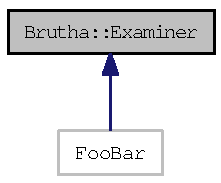
\includegraphics[width=71pt]{classBrutha_1_1Examiner__inherit__graph}
\end{center}
\end{figure}
\subsection*{Public Member Functions}
\begin{CompactItemize}
\item 
\hypertarget{classBrutha_1_1Examiner_cdb51602511acc68751aca346e6381f5}{
virtual bool \textbf{operator()} (\hyperlink{classBrutha_1_1TraversalCallback}{TraversalCallback} \&)=0}
\label{classBrutha_1_1Examiner_cdb51602511acc68751aca346e6381f5}

\end{CompactItemize}


\subsection{Detailed Description}
An abstract class from which each examiner object must inherit. 

Examiners are used to process cube states that are generated by \hyperlink{classBrutha_1_1Traversal}{Traversal} objects.

\begin{Desc}
\item[See also:]\hyperlink{classBrutha_1_1Traversal}{Traversal} \end{Desc}


The documentation for this class was generated from the following file:\begin{CompactItemize}
\item 
src/Examiner.h\end{CompactItemize}

\hypertarget{classBrutha_1_1ReverseSequence}{
\section{Brutha::ReverseSequence Class Reference}
\label{classBrutha_1_1ReverseSequence}\index{Brutha::ReverseSequence@{Brutha::ReverseSequence}}
}
Some of traversal techniques create sequences on demand, by using backtracking.  


{\tt \#include $<$ReverseSequence.h$>$}

Inheritance diagram for Brutha::ReverseSequence:\nopagebreak
\begin{figure}[H]
\begin{center}
\leavevmode
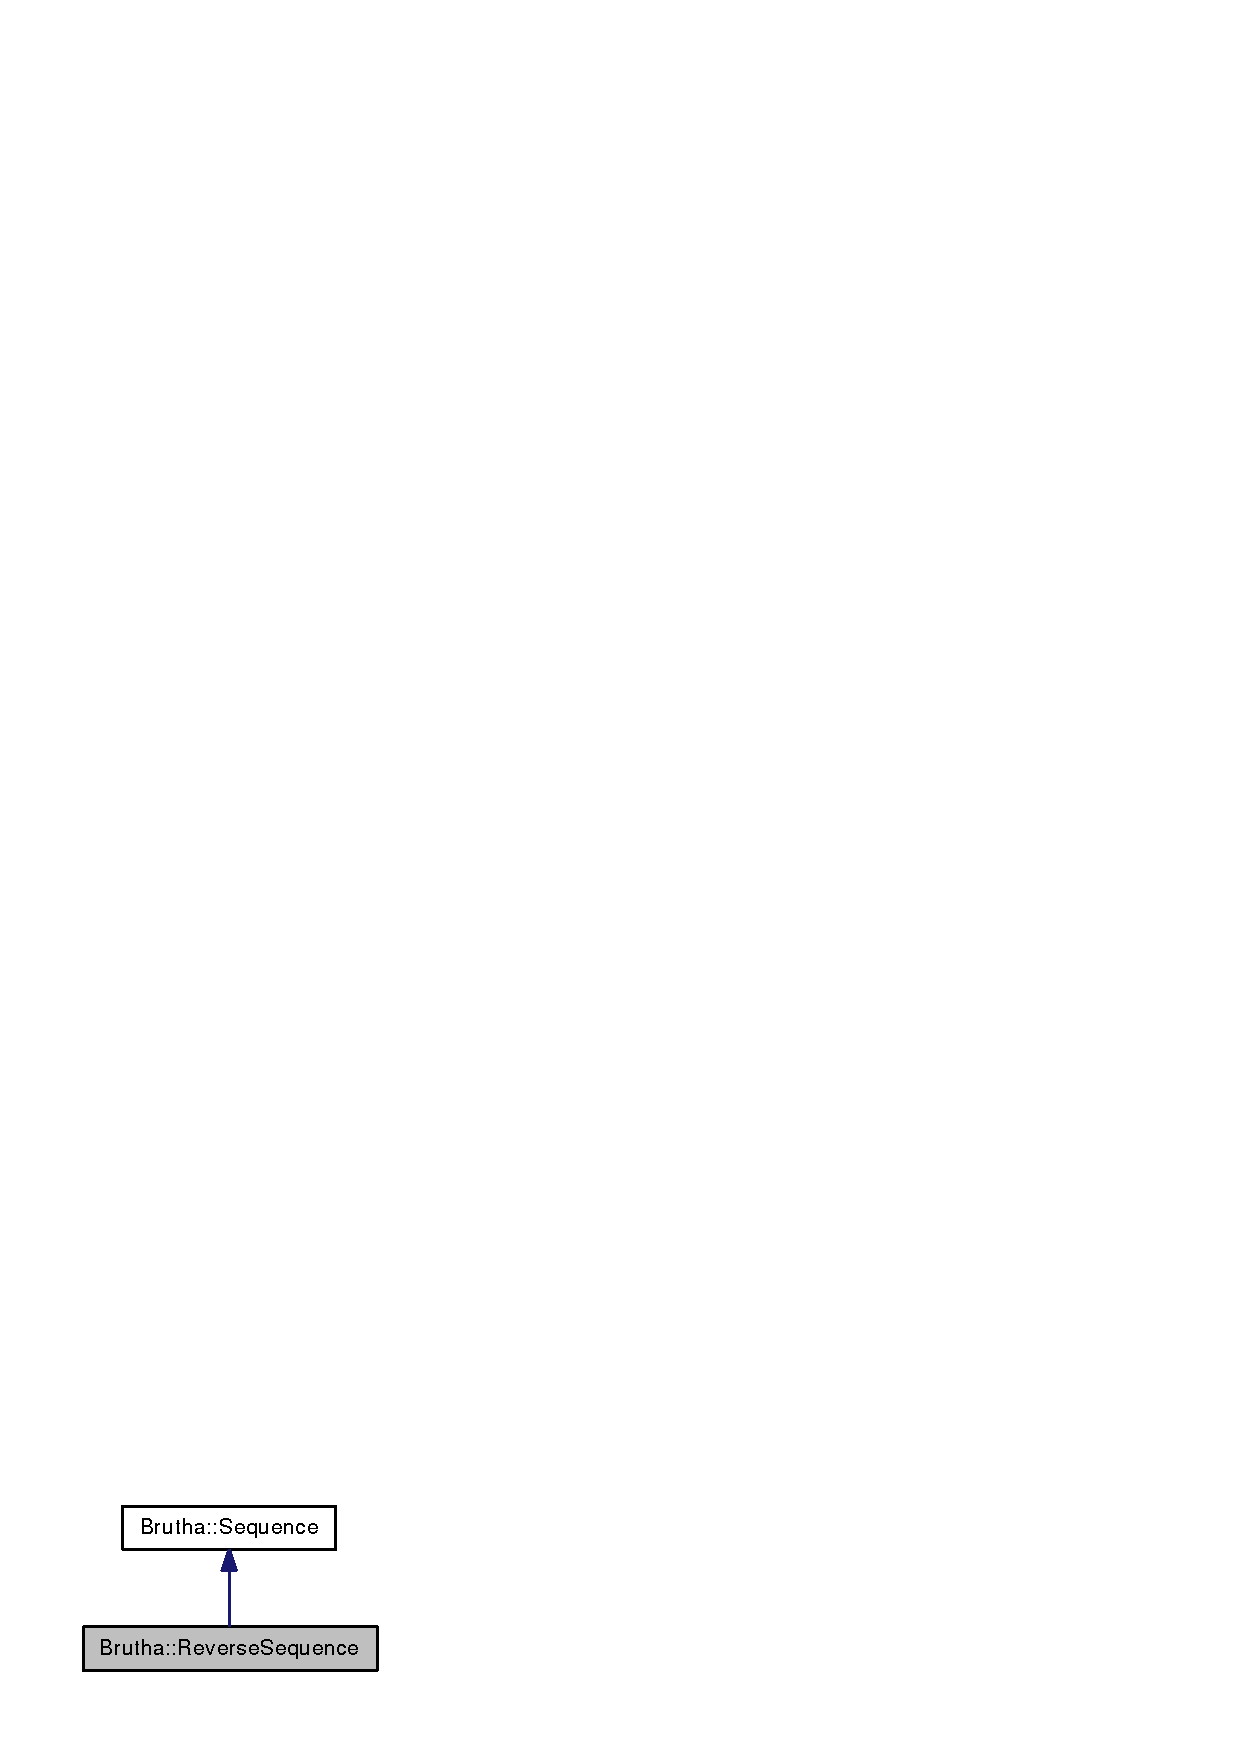
\includegraphics[width=92pt]{classBrutha_1_1ReverseSequence__inherit__graph}
\end{center}
\end{figure}
Collaboration diagram for Brutha::ReverseSequence:\nopagebreak
\begin{figure}[H]
\begin{center}
\leavevmode
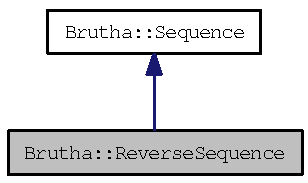
\includegraphics[width=92pt]{classBrutha_1_1ReverseSequence__coll__graph}
\end{center}
\end{figure}
\subsection*{Public Member Functions}
\begin{CompactItemize}
\item 
\hypertarget{classBrutha_1_1ReverseSequence_b82a0c24091e2ebff7f7a06f8b25e7d5}{
\textbf{ReverseSequence} (const vector$<$ Move $>$ \&\_\-moves)}
\label{classBrutha_1_1ReverseSequence_b82a0c24091e2ebff7f7a06f8b25e7d5}

\item 
\hypertarget{classBrutha_1_1ReverseSequence_604e7ea40ce375a3d28e1dd46dd5079d}{
virtual const Move \& \hyperlink{classBrutha_1_1ReverseSequence_604e7ea40ce375a3d28e1dd46dd5079d}{operator\mbox{[}$\,$\mbox{]}} (int index) const }
\label{classBrutha_1_1ReverseSequence_604e7ea40ce375a3d28e1dd46dd5079d}

\begin{CompactList}\small\item\em Returns a Move object at the given position. \item\end{CompactList}\end{CompactItemize}


\subsection{Detailed Description}
Some of traversal techniques create sequences on demand, by using backtracking. 

They, therefore, produce 'reverse' sequences.

This is moment when the \hyperlink{classBrutha_1_1ReverseSequence}{ReverseSequence} comes to play. 

The documentation for this class was generated from the following files:\begin{CompactItemize}
\item 
src/ReverseSequence.h\item 
src/ReverseSequence.cpp\end{CompactItemize}

\hypertarget{classBrutha_1_1Sequence}{
\section{Brutha::Sequence Class Reference}
\label{classBrutha_1_1Sequence}\index{Brutha::Sequence@{Brutha::Sequence}}
}
\hyperlink{classBrutha_1_1Sequence}{Sequence} represents a certain move sequence.  


{\tt \#include $<$Sequence.h$>$}

Inheritance diagram for Brutha::Sequence:\nopagebreak
\begin{figure}[H]
\begin{center}
\leavevmode
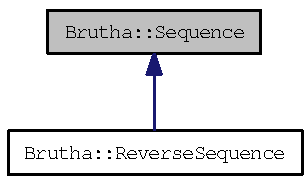
\includegraphics[width=92pt]{classBrutha_1_1Sequence__inherit__graph}
\end{center}
\end{figure}
\subsection*{Public Member Functions}
\begin{CompactItemize}
\item 
\hypertarget{classBrutha_1_1Sequence_642c0d4d05d18ece53275f58b7120a18}{
\textbf{Sequence} (const vector$<$ Move $>$ \&\_\-moves)}
\label{classBrutha_1_1Sequence_642c0d4d05d18ece53275f58b7120a18}

\item 
virtual int \hyperlink{classBrutha_1_1Sequence_9e2aa4c6db6063aff5247f2cd5e7b7df}{size} () const 
\begin{CompactList}\small\item\em Returns a size of the underlying storage. \item\end{CompactList}\item 
\hypertarget{classBrutha_1_1Sequence_830bc00f3067f33664f91d519eeb80f2}{
virtual const Move \& \hyperlink{classBrutha_1_1Sequence_830bc00f3067f33664f91d519eeb80f2}{operator\mbox{[}$\,$\mbox{]}} (int index) const }
\label{classBrutha_1_1Sequence_830bc00f3067f33664f91d519eeb80f2}

\begin{CompactList}\small\item\em Returns a Move object at the given position. \item\end{CompactList}\item 
\hypertarget{classBrutha_1_1Sequence_33967587aa561719e322594d2247f63f}{
virtual void \textbf{push} (Move move)}
\label{classBrutha_1_1Sequence_33967587aa561719e322594d2247f63f}

\item 
\hypertarget{classBrutha_1_1Sequence_5e86148bf39752cef9054ecd7354d9d0}{
virtual const Move \& \textbf{pop} ()}
\label{classBrutha_1_1Sequence_5e86148bf39752cef9054ecd7354d9d0}

\item 
\hypertarget{classBrutha_1_1Sequence_599b970cf400ee90b250ea9b578af8f4}{
virtual void \textbf{clear} ()}
\label{classBrutha_1_1Sequence_599b970cf400ee90b250ea9b578af8f4}

\item 
\hypertarget{classBrutha_1_1Sequence_43951830faef8f02b8eff4b0eaabd0b8}{
virtual int \textbf{getQtmMetric} () const }
\label{classBrutha_1_1Sequence_43951830faef8f02b8eff4b0eaabd0b8}

\item 
\hypertarget{classBrutha_1_1Sequence_3e2ec4f84a589c4ac3cfb2d5810b1a0b}{
virtual int \textbf{getHtmMetric} () const }
\label{classBrutha_1_1Sequence_3e2ec4f84a589c4ac3cfb2d5810b1a0b}

\item 
virtual string \hyperlink{classBrutha_1_1Sequence_a33a3b258707feb3b35e94b780b22ee4}{format} () const 
\begin{CompactList}\small\item\em Formats a \hyperlink{classBrutha_1_1Sequence}{Sequence} to a human-readable form. \item\end{CompactList}\end{CompactItemize}
\subsection*{Protected Attributes}
\begin{CompactItemize}
\item 
\hypertarget{classBrutha_1_1Sequence_e462d084fb3674cd8667cef4fdd9d7d8}{
vector$<$ char $>$ \textbf{storage}}
\label{classBrutha_1_1Sequence_e462d084fb3674cd8667cef4fdd9d7d8}

\item 
\hypertarget{classBrutha_1_1Sequence_1a72ab6f5624bebb3ec99ff463f7eccd}{
const vector$<$ Move $>$ \& \textbf{moves}}
\label{classBrutha_1_1Sequence_1a72ab6f5624bebb3ec99ff463f7eccd}

\end{CompactItemize}


\subsection{Detailed Description}
\hyperlink{classBrutha_1_1Sequence}{Sequence} represents a certain move sequence. 

\subsection{Member Function Documentation}
\hypertarget{classBrutha_1_1Sequence_a33a3b258707feb3b35e94b780b22ee4}{
\index{Brutha::Sequence@{Brutha::Sequence}!format@{format}}
\index{format@{format}!Brutha::Sequence@{Brutha::Sequence}}
\subsubsection[{format}]{\setlength{\rightskip}{0pt plus 5cm}string Brutha::Sequence::format () const\hspace{0.3cm}{\tt  \mbox{[}virtual\mbox{]}}}}
\label{classBrutha_1_1Sequence_a33a3b258707feb3b35e94b780b22ee4}


Formats a \hyperlink{classBrutha_1_1Sequence}{Sequence} to a human-readable form. 

\begin{Desc}
\item[Returns:]string representation. \end{Desc}
\hypertarget{classBrutha_1_1Sequence_9e2aa4c6db6063aff5247f2cd5e7b7df}{
\index{Brutha::Sequence@{Brutha::Sequence}!size@{size}}
\index{size@{size}!Brutha::Sequence@{Brutha::Sequence}}
\subsubsection[{size}]{\setlength{\rightskip}{0pt plus 5cm}int Brutha::Sequence::size () const\hspace{0.3cm}{\tt  \mbox{[}virtual\mbox{]}}}}
\label{classBrutha_1_1Sequence_9e2aa4c6db6063aff5247f2cd5e7b7df}


Returns a size of the underlying storage. 

For more apropriate measure of the number of moves in the sequence, use getQtmMetric and getHtmMetric.

\begin{Desc}
\item[See also:]getHtmMetric 

getQtmMetric \end{Desc}


The documentation for this class was generated from the following files:\begin{CompactItemize}
\item 
src/Sequence.h\item 
src/Sequence.cpp\end{CompactItemize}

\hypertarget{classBrutha_1_1Traversal}{
\section{Brutha::Traversal Class Reference}
\label{classBrutha_1_1Traversal}\index{Brutha::Traversal@{Brutha::Traversal}}
}
An abstract class for \hyperlink{classBrutha_1_1Traversal}{Traversal} objects.  


{\tt \#include $<$Traversal.h$>$}

Inheritance diagram for Brutha::Traversal:\nopagebreak
\begin{figure}[H]
\begin{center}
\leavevmode
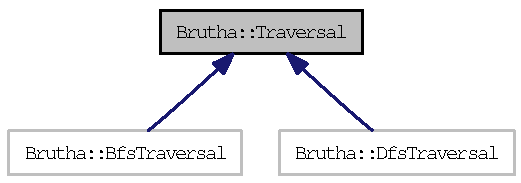
\includegraphics[width=143pt]{classBrutha_1_1Traversal__inherit__graph}
\end{center}
\end{figure}
\subsection*{Public Member Functions}
\begin{CompactItemize}
\item 
virtual void \hyperlink{classBrutha_1_1Traversal_67ab6c006a71670a85bf44e402929d01}{traverse} (Cube state, \hyperlink{classBrutha_1_1Examiner}{Examiner} \&examiner)=0
\begin{CompactList}\small\item\em Performs the traversal. \item\end{CompactList}\end{CompactItemize}


\subsection{Detailed Description}
An abstract class for \hyperlink{classBrutha_1_1Traversal}{Traversal} objects. 

These objects traverse through the whole 2x2x2 state universe using a defined technique.

Each of these states is then encapsulated in \hyperlink{classBrutha_1_1TraversalCallback}{TraversalCallback} and passed to \hyperlink{classBrutha_1_1Examiner}{Examiner} object, which is user-provided.

\begin{Desc}
\item[See also:]\hyperlink{classBrutha_1_1TraversalCallback}{TraversalCallback} 

\hyperlink{classBrutha_1_1Examiner}{Examiner} \end{Desc}


\subsection{Member Function Documentation}
\hypertarget{classBrutha_1_1Traversal_67ab6c006a71670a85bf44e402929d01}{
\index{Brutha::Traversal@{Brutha::Traversal}!traverse@{traverse}}
\index{traverse@{traverse}!Brutha::Traversal@{Brutha::Traversal}}
\subsubsection[{traverse}]{\setlength{\rightskip}{0pt plus 5cm}virtual void Brutha::Traversal::traverse (Cube {\em state}, \/  {\bf Examiner} \& {\em examiner})\hspace{0.3cm}{\tt  \mbox{[}pure virtual\mbox{]}}}}
\label{classBrutha_1_1Traversal_67ab6c006a71670a85bf44e402929d01}


Performs the traversal. 

\begin{Desc}
\item[Parameters:]
\begin{description}
\item[{\em state}]beginning state. \item[{\em examiner}]user-provided object which examines each visited state. \end{description}
\end{Desc}


The documentation for this class was generated from the following file:\begin{CompactItemize}
\item 
src/Traversal.h\end{CompactItemize}

\hypertarget{classBrutha_1_1TraversalCallback}{
\section{Brutha::TraversalCallback Class Reference}
\label{classBrutha_1_1TraversalCallback}\index{Brutha::TraversalCallback@{Brutha::TraversalCallback}}
}
An abstract class for information chunks that are given to \hyperlink{classBrutha_1_1Examiner}{Examiner} objects by TraveRsal objects.  


{\tt \#include $<$TraversalCallback.h$>$}

Inheritance diagram for Brutha::TraversalCallback:\nopagebreak
\begin{figure}[H]
\begin{center}
\leavevmode
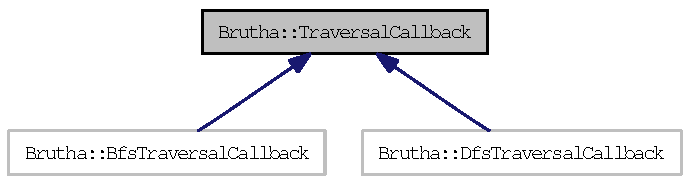
\includegraphics[width=183pt]{classBrutha_1_1TraversalCallback__inherit__graph}
\end{center}
\end{figure}
\subsection*{Public Member Functions}
\begin{CompactItemize}
\item 
virtual Cube \hyperlink{classBrutha_1_1TraversalCallback_c037795e35fc6b1a2c65cb1e0e976356}{getState} ()=0
\begin{CompactList}\small\item\em Returns current cube state.A. \item\end{CompactList}\item 
virtual const \hyperlink{classBrutha_1_1Sequence}{Sequence} \& \hyperlink{classBrutha_1_1TraversalCallback_8946d090513db014bbf7b542dc70866c}{getSequence} ()=0
\begin{CompactList}\small\item\em Returns a sequence of moves that leads from the traversal beginning state to the current one. \item\end{CompactList}\item 
\hypertarget{classBrutha_1_1TraversalCallback_b0c7e8d859f10ad580c805e93555443d}{
virtual const Move \& \textbf{getParentMove} ()=0}
\label{classBrutha_1_1TraversalCallback_b0c7e8d859f10ad580c805e93555443d}

\end{CompactItemize}


\subsection{Detailed Description}
An abstract class for information chunks that are given to \hyperlink{classBrutha_1_1Examiner}{Examiner} objects by TraveRsal objects. 

\begin{Desc}
\item[See also:]\hyperlink{classBrutha_1_1Traversal}{Traversal} 

\hyperlink{classBrutha_1_1Examiner}{Examiner} \end{Desc}


\subsection{Member Function Documentation}
\hypertarget{classBrutha_1_1TraversalCallback_8946d090513db014bbf7b542dc70866c}{
\index{Brutha::TraversalCallback@{Brutha::TraversalCallback}!getSequence@{getSequence}}
\index{getSequence@{getSequence}!Brutha::TraversalCallback@{Brutha::TraversalCallback}}
\subsubsection[{getSequence}]{\setlength{\rightskip}{0pt plus 5cm}virtual const {\bf Sequence}\& Brutha::TraversalCallback::getSequence ()\hspace{0.3cm}{\tt  \mbox{[}pure virtual\mbox{]}}}}
\label{classBrutha_1_1TraversalCallback_8946d090513db014bbf7b542dc70866c}


Returns a sequence of moves that leads from the traversal beginning state to the current one. 

\begin{Desc}
\item[Note:]This operation can be time consuming, depending on the travelsal technique. Use it sparingly.\end{Desc}
\begin{Desc}
\item[Returns:]a \hyperlink{classBrutha_1_1Sequence}{Sequence} object.\end{Desc}
\begin{Desc}
\item[See also:]\hyperlink{classBrutha_1_1TraversalCallback_c037795e35fc6b1a2c65cb1e0e976356}{getState} 

\hyperlink{classBrutha_1_1Sequence}{Sequence} \end{Desc}
\hypertarget{classBrutha_1_1TraversalCallback_c037795e35fc6b1a2c65cb1e0e976356}{
\index{Brutha::TraversalCallback@{Brutha::TraversalCallback}!getState@{getState}}
\index{getState@{getState}!Brutha::TraversalCallback@{Brutha::TraversalCallback}}
\subsubsection[{getState}]{\setlength{\rightskip}{0pt plus 5cm}virtual Cube Brutha::TraversalCallback::getState ()\hspace{0.3cm}{\tt  \mbox{[}pure virtual\mbox{]}}}}
\label{classBrutha_1_1TraversalCallback_c037795e35fc6b1a2c65cb1e0e976356}


Returns current cube state.A. 

\begin{Desc}
\item[Returns:]Puzzle state. \end{Desc}


The documentation for this class was generated from the following file:\begin{CompactItemize}
\item 
src/TraversalCallback.h\end{CompactItemize}

\printindex
\end{document}
